\documentclass[12pt]{article}

% Load packages
\usepackage[top=1in, bottom=1in, left=1in, right=1in]{geometry}
\usepackage{graphics}
\usepackage[pdftex]{graphicx}
\usepackage{epsfig}
\usepackage{epsf}
\usepackage{epstopdf}
\usepackage{mathrsfs}
\usepackage{amsmath}
\usepackage{amssymb}
\usepackage{textcomp}
\usepackage[scaled=.90]{helvet} % Helvetica (currently not used)
\usepackage[]{lineno} % For line numbers
\usepackage{natbib}
\usepackage{sidecap}

% Define new commands and definitions
\def\ds{\displaystyle}
\def\d{\partial}
\newcommand{\rr}{\mathbb{R}}
\newcommand{\zz}{\mathbb{Z}}
\newcommand{\nn}{\mathbb{N}}
\newcommand{\ee}{\mathscr{E}}
\newcommand{\mb}{\mathbf}
\newcommand{\ol}{\overline}

% Text formatting
\linespread 2	
\linenumbers

\title{Escape direction does not matter for some fish prey}
\author{Matthew J. McHenry, Alberto Soto}
%\date{}                                           % Activate to display a given date or no date

\begin{document}
\DeclareGraphicsExtensions{.eps,.pdf,.png,.gif,.jpg,.ps}

\maketitle

\pagebreak


% ABSTRACT
% --------------------------------------------------------------------------------
\begin{abstract}

Although predator evasion is generally considered important to the ecology and evolution of fish prey species, the strategies that permit prey survival are largely unclear. A theoretical framework for understanding these interactions is offered by pursuit models that determine the optimal direction that prey may move to maximize their distance from a predator. We examined how deviation from optimal strategy affects the ability of prey to evade predators, as indicated by the minimum distance over time between a predator and prey. Using numerical and analytical approaches, we found that escape direction matters little when predators are more than 10 times the speed of a prey because locomotion by the predator overwhelms that of the prey. When the prey are faster than predators, then the escape direction has no effect on escape performance for a broad range of escape angles. This is the case for zebrafish larvae (\textit{Danio rerio}), which achieve a high velocity with an escape response that is executed when predator fish attempt a slow approach during suction feeding. The optimal evasion strategy is therefore most biologically meaningful when the predator is faster than the prey, but by less than an order of magnitude. In this regime, the accuracy of the predator is also a major determinant of a prey's ability to evade an attack.

\end{abstract}

\pagebreak


% --------------------------------------------------------------------------------
\section{Introduction}
\label{intro}

Biologists have long--appreciated the importance of predation in the ecology and evolution of prey species. This subject is extensive enough to fill the pages of books with the fascinating diversity of strategies that prey use to avoid encounters with predators \citep[e.g.][]{Ruxton:2004vb} or to defend themselves when discovered \citep[e.g.][]{Emlen:2014wb, Evans:1990va}. In contrast, our understanding for how prey evade capture by locomotion is relatively rudimentary. Although biomechanical studies commonly speculate on the importance of locomotor performance to survival, relatively few have tested what aspect of locomotion are most meaningful in these interactions. Studies that have explored this subject \citep[reviewed by][]{Domenici:2011tv} underscore the common-sense notion that the direction of an escape matters to a prey's survival. The present paper examines pursuit models that consider the strategic implications of a prey fish's escape direction. We offer a new interpretation of a model for piscivorous interactions \citep{Weihs:1984tb} and relate its predictions to experimental measurements of larval zebrafish (\textit{Danio rerio}) \citep{Stewart:2014cm}.

Pursuit models are an area of game theory that offers a basis for examining locomotor behavior in strategic terms. There is recent interest in revisiting these models \citep[e.g.][]{Howland:1974, Weihs:1984tb} with experimental studies that consider the behavior of both predators and prey. This includes work on running vertebrates \citep[e.g.][]{Wilson:2014fd}, birds \citep[e.g.][]{Hedenstrom:2001do, Kullberg:1998ur} and bats \citep[e.g.][]{Ghose:2006dk} in flight, running insects \citep{Domenici:2008kra}, flying insects \citep[e.g.][]{Combes:2012eta}, and swimming zooplankton \citep[e.g.][]{Arnott:1999wx} and fishes \citep[e.g.][]{Domenici:2000un}. These efforts offer the potential to reveal how sensory and motor systems govern the outcome of predator--prey interactions. 

A piscivorous interaction offers some advantages as a model for examining the sensory-motor basis of predator evasion. In many cases, this interaction can be easily studied in a laboratory. Under artificial conditions, many predatory fishes will attempt to feed on prey and the prey will initiate a 'fast-start' escape response (Fig. \ref{prey_prey}). Both players operate with motion that is largely two-dimensional and therefore relatively simple to measure and describe. Zebrafish exhibit both predator evasion and predatory behavior in the lab \citep{Stewart:2013bh} and it is a species that offers a growing wealth of understanding in physiology and neuroscience \citep[e.g.][]{McLean:2011gi, Briggs:2002uf} that may be leveraged for mechanistic insight on predator--prey interactions. In addition, fish offer one of the few biological pursuit systems that have been modeled. Weihs and Webb adapted classic differential game theory to model the optimal escape direction for a prey fish \citep{Weihs:1984tb}. This offers specific predictions of swimming trajectories that may be tested with kinematic measurements. Our present analysis considers this model in detail and offers some new interpretations of its predictions.

A variety of interpretations have been offered for the failure of a prey animal to conform to the optimal strategy predicted by a pursuit model. The model's assumptions could be violated by the system. For example, a prey fish cannot move in an optimal direction that maximizes its distance from a predator if it cannot detect the predator's speed \citep{Weihs:1984tb}. An alternative explanation is the protean hypothesis, which suggests that prey should move in a variety of directions so that they are unpredictable in the experience of a predator \citep{Domenici:2011tv, Humphries:1970hy}. This idea is distinct from an individual moving in circuitous path, such as moths that evade bats (CITE), because the escape response in fish is a ballistic motion in a particular direction \citep{D:1973up}. 

Interpretations of prey motion have generally not considered the effect of deviating from optimal strategy. For example, it is not clear whether an escape that is 5\textdegree\hspace{0.5pt} from the optimum predicted by Weihs and Webb (1984) has a major or negligible effect on its escape. If evasive performance is insensitive to differences in strategy, then the prey has the permission to move in a random, or constrained, direction with little threat of a penalty. Therefore the present study revisits the mathematics of the Weihs and Webb (1984) model to examine the implications of deviation from optimal strategy. This allowed for an interpretation of measured responses in zebrafish in terms of evasive performance.

% --------------------------------------------------------------------------------
\section{Optimal prey strategy}
\label{opt_strategy}

The Homicidal Chauffeur is the colorful title for a pursuit game that has been applied to predator--prey interactions \citep{Isaacs:1965va}. Pursuit games consider the trajectories of both players and thereby address the effects of directional decision--making to the outcome of an interaction. Weihs and Webb (1984) adopted the Homicidal Chauffeur to model the responses of a prey fish that encounters a predator fish. Here we offer a brief review of this model as a means to explain the basis for our own interpretations of prey strategy, though a more complete derivation is presented in the original study \citep{Weihs:1984tb}.

The payoff is a quantity used in game models to define the beneficial or detrimental consequences of playing with a particular strategy \citep{Webb:2007hg}. For considering evasive strategy, the payoff has been defined as the minimum distance between predator and prey. This quantity reflects the instance where the predator has the best opportunity to capture the prey (Weihs and Webb, 1984). Therefore, the optimal strategy for a prey is defined as the escape angle that yields the greatest minimum distance.

Predicting the distance between predator and prey requires relatively few parameters under some simplifying assumptions. In the rapid events of a predatory strike, it is reasonable to approximate the predator's motion as a constant speed, $U$. One may further assume that the prey initiates its escape at a position ahead of the predator with a fast start that may be approximated with a constant speed, $V$. Therefore, the following equation defines the distance between predator and prey over time:
%
\begin{equation}
D^2 = ((X_0 - Ut) + Vt\cos\alpha)^2 + (Vt\sin\alpha)^2,
\label{dist}
\end{equation}
%
where $\alpha$ is the escape angle and $X_0$ is the starting position of the prey. Note that the prey's motion is described in a frame of reference set by the predator. In particular, its origin is positioned at the predator's mouth at $t= 0$, but it does not move with the predator, and the $X$-axis is coincident with the predator's heading (Fig. 1A). 

Given the definition of the payoff for this model, only the closest distance between predator and prey matters. The first step toward finding this minimum is to calculate the time, $t_{\text{min}}$,  at which it occurs. This may be found from the root of the first derivative of Eqn. \ref{dist} with respect to time, which yields the following solution:
%
\begin{equation}
t_{\text{min}} = \frac{X_0}{V} \frac{K-\cos\alpha}{1-2 K\cos\alpha+K^2},
\label{eq33weihs}	
\end{equation}
%
where $K$ indicates the speed of the predator relative to the prey ($K = U/V$). The authors observed that this equation yields negative values of time where $K<1$ and is therefore only useful when the predator is faster than the prey. The minimum distance was consequently determined for $K>1$ by solving for distance (Eqn. \ref{dist}) at $t_{\text{min}}$:
%
\begin{equation}
\ol D_{\text{min}}^2 = \frac{D_{\text{min}}^2}{X_0^2} = \frac{\sin^2\alpha}{K^2 - 2K \cos\alpha + 1},
\label{dmin}
\end{equation}
where $\ol D_{\text{min}}$ is the minimum distance normalized by the starting position of the prey.

Finally, the optimal strategy for the prey may be determined by finding the escape angle that yields the greatest minimum distance. This occurs where the derivative of Eqn. \ref{dmin} with respect to $\alpha$ is equal to zero, which is explicitly described by the following equation:
%
\begin{equation}
0 = \frac{\d \ol{D}^2_{\text{min}}}{\d \alpha} = \frac{2\sin\alpha \cos\alpha (K^2 -2 K \cos\alpha+1)-2 K \sin^3\alpha}{(K^2-2 K \cos\alpha + 1)^2}. 
\label{eq37weihs}
\end{equation}
%
Among the solutions that satisfy this equation, Weihs and Webb proposed that the following indicates the optimal strategy when the predator is faster than the prey ($K>1$):
%
\begin{equation}
\alpha_{\text{opt}} = \pm \arccos K^{-1}. 
\label{K>1}
\end{equation}
%
For relatively fast prey ($K\leq1$), the authors further suggested that the optimal solution consists of swimming directly away from the predator ($\alpha = 0$). Therefore, for any predator speed, this model offers predictions for how a prey can vary the direction of its escape to maximize its chances for survival by creating distance from a predator. 

% --------------------------------------------------------------------------------
\section{When optimal strategy matters}

An optimum is less meaningful if it corresponds to a shallow peak in performance or defines a local peak that is much smaller than the global maximum. We considered whether these conditions exist in evasion strategy by calculating how the payoff in this pursuit model, the minimum distance \citep{Weihs:1984tb}, varies with escape angle and relative speed of the predator. Therefore, we were intent on examining a performance landscape of prey strategy. As an alternative to analytical mathematics (Eqn. \ref{dmin}), we first formulated this landscape with a numerical approach that is simple enough to execute in a spreadsheet, but which we implemented in Matlab (MathWorks, Natick, MA, USA). This was done by defining a series of time values at an equal interval to provide the basis of calculations of the positions of the predator ($X_{\text{pred}} = Ut$, $Y_{\text{pred}} = 0$) and prey ($X_{\text{prey}}=Vt\cos\alpha,Y_{\text{prey}}=Vt\sin\alpha$). The minimum value of the distance between them was determined in this way for variable escape angle and predator speed, over a range of $K$ and $\alpha$ values (Fig. \ref{weihs_topo}B). This yielded results that were coincident with the analytical equation for $\ol D_{\text{min}}$ formulated by Weihs and Webb (1984) for relatively fast predators ($K>1$, Eqn. \ref{dmin}). However, the value of the numerical calculations is that they allowed us to examine variation in the minimum distance for slower predators (i.e. $K<1$) as well. The resulting performance landscape (Fig. \ref{weihs_topo}B) illustrates how the minimum distance varies over a broad range of values in the speed of the predator and escape angle of the prey.

This result suggests that the fast start is unlikely to be effective at any escape angle when a prey is approached by a very fast predator. For example, if a predator is an order of magnitude faster than its prey (i.e. $K=10$), then the prey can do no better than displace its body by $10\%$ of its initial distance from the predator (Fig. \ref{weihs_topo}B). In addition, differences in escape angle have little effect on the minimum distance. An escape that is  24.5\textdegree\hspace{2pt} larger or smaller than the optimum yields a minimum distance that is less than the value at the optimum by 0.1 (i.e. 1\% of the starting position of the prey). These metrics become increasingly unfavorable for the prey when approached by an even faster predator (Fig. \ref{weihs_topo}B). At these speeds, inaccuracy in the feeding strike is likely a more decisive factor to prey survivorship than anything the prey may do in response.

A very different picture emerges when one considers prey that move more quickly than their predators (i.e. $K<1$). This condition occurs when predators brake or glide slowly on their approach toward a prey \citep{Higham:2007go, Higham:2005iu} while the prey initiates a rapid escape. For a variety of escape angles, the fast start of these prey cause the predator to reach no closer than the starting distance (i.e. $\ol D_{\text{min}}=1$, Fig. \ref{weihs_topo}B). In order to define the bounds of this domain, it is useful to consider the first derivative of the distance function with respect to time:
%
\begin{equation}
\frac{\d D^2}{\d t}= 2(t(U^2+V^2) - UX_0 + V(X_0-2tU)\cos\alpha).
\label{distderivative}
\end{equation}  
%
A prey achieves an optimal escape ($\ol D_{\text{min}}=1$) when the distance function only increases as a function of time (i.e. $\frac{\d D^2}{\d t}\geq0$). This holds true for $\alpha=0$, which Weihs and Webb proposed as the optimal direction (Weihs and Webb, 1984). However, it also holds true that distance increases for another solution to Eqn. \ref{eq37weihs} ($\alpha=\arccos K$) and all values in between. Therefore, the following defines the domain of optimal directions when the prey is faster than the predator ($K<1$):
%
\begin{equation}
0 \leq \alpha \leq \pm \arccos(K).
\label{anglerange}
\end{equation}
%
Therefore, if the escape response of a prey is capable of exceeding the approach speed of the predator, then a wide range of angles yield equally successful escapes for the prey and thereby define a performance plateau. 

The domain where optimal the optimal strategy is most meaningful resides between where the prey and predator are equivalent in speed and where the predator is an order of magnitude faster ($1<K<10$). In this domain, prey are capable of attaining appreciable minimum distance values and there is a penalty for deviating from the optimal angle (Fig. \ref{weihs_topo}B). Therefore, a prey fish has an incentive to conform to the optimal prediction when encountering a slightly faster predator.

% --------------------------------------------------------------------------------
\section{Comparing models with measurements}

We were interested examine whether optimal strategy matters in our measurements of predator-prey interactions. We addressed this issue with some of our recent experimental measurements on larval zebrafish that encountered adult predators of the same species \citep{Stewart:2014cm}. These experiments used a robot to simulate the approach of a predator toward prey in the dark and we recorded the position at which the prey responded and the direction of the fast start. The bow wave of flow around the predator's body stimulated the lateral line system of the prey to initiate a fast start. 

As detailed above, the predictions of the model depend on the speed of the predator relative to the prey. The approach speed, and consequently $K$, was varied to span the range of values observed for a live predator \citep{Stewart:2013bh}. Our calculations of $K$ used a prey speed ($U=22 \text{ cm s}^{-1}$) from the literature that approximates the maximum speed attained during a fast start for larvae of this species \citep{Budick:2000wrb, Muller:2004hp}. As a consequence of the relatively slow approach made by these suction-feeding predators, the prey had the potential to move faster at all approach speeds, which yielded $K$-values that were uniformly less than unity (Fig. \ref{our_topo}A).

One discrepancy between the model and our experiments was that the majority of prey fish did not initiate the fast start at a position directly along the heading of the predator robot. This condition has biological relevance because it corresponds to a situation where a predator fails to align its approach with a prey's position. We therefore modified the Weihs and Webb model by adding a lateral initial position of the prey to the distance function (Eqn. \ref{dist}) and then following the same procedure (as in Eqns. \ref{eq33weihs}--\ref{dmin}) to arrive at a minimum distance function. We found that this equation was simplified by the use of polar coordinates, which yielding the following:
%
\begin{equation}
\ol{D}^2_{\text{min}}= \ds\frac{{D}^2_{\text{min}}}{R_0^2 }=
\ds\frac{\left ( \sin(\alpha - \theta_0) + K \sin \theta_0 \right )^2}{K^2-2 K \cos \alpha +1} 
\label{Dmin_polar}
\end{equation}
%
where $R_0$ and $\theta_0$ are the initial radial and angular positions of the prey relative to the mouth of the predator (Fig. \ref{weihs_topo}A). Numerical solutions to this equation show a broad range of angular positions and escape angles that define a performance plateau where $D_{\text{min}}=1$ (Fig. \ref{our_topo}B). We found the margins of this plateau using a similar procedure as outlined above. Specifically, we solved for the conditions where the derivative of the minimum distance with respect to $\alpha$ was equal to zero:
%
\begin{equation}
0 = \frac{\d \ol{D}^2_{\text{min}}}{\d \alpha} = 
\frac{2(K \cos \alpha - 1)(K\cos \theta_0 - \cos(\alpha - \theta_0))(K\sin \theta_0 + \sin(\alpha -\theta_0))}
{(K^2 - 2K \cos \alpha + 1)^2}
\label{DminDalpha}
\end{equation} 
%
One can find the solutions that satisfy this equation by setting the terms in the numerator equal to zero. One finds that the solution for $K>1$ is similar to Eqn. \ref, though angular position determines the sign of the optimal angle: $\alpha_{\text{opt}}=arccos{K^{-1}}$ for $\theta_0>0$ and $\alpha_{\text{opt}}=-arccos{K^{-1}}$ for $\theta_0<0$. Therefore, the same optimal direction exists when the predator is faster, irrespective of the starting position of the prey. When the prey is faster, we found that the escape angle is equally effective (i.e. $\ol D_{\text{min}}=1$) for a broad range of values (Eqn. \ref{anglerange}), as detailed above. This result holds true when prey are positioned lateral to the predator, but this performance plateau depends on the initial angular position of the prey. We found that the bounds of this plateau in performance where $\ol D_{\text{min}}=1$ among the solutions that satisfy Eqn. \ref{DminDalpha} for $K<1$:
%
\begin{equation}
\alpha_{\text{opt}} = \theta_0 \pm \arccos(K \cos \theta_0).
\end{equation}
%
This relationship demonstrates how the performance plateau reduces in area with increasing predator speed (Fig. \ref{our_topo}B). Therefore, fewer combinations of starting positions and escape angles yield equivalent escape performance for faster predators.

Using this formulation of the pursuit model, we evaluated how the measured responses of prey compared to the model predictions (Fig. \ref{our_topo}C). This comparison revealed that the vast majority of larvae responded at a position and with an escape direction that was predicted to yield maximal performance  ($\ol D_{\text{min}}=1$). This was true even at the fastest predator approach speed, where a larger number of individuals responded outside of the plateau.  According to the model's predictions, the large variation in observed escape direction incurs no penalty in the evasive performance of most larvae. 

% --------------------------------------------------------------------------------
\section{Predator strategy}

Although the present pursuit models are formulated with a focus on prey fish, they provide the opportunity to consider the strategy of fish predators. It first merits pointing out that the payout considered presently is normalized by the initial response distance of the prey (Figs. \ref{weihs_topo}--\ref{our_topo}). Therefore, the absolute distance traversed by a prey is predicted to be proportional to the initial response distance. The predator may act to minimize this distance with a slower approach, which will serve to reduce the stimulus intensity for the visual (CITE) and lateral line (CITE) systems. This is one benefit to the braking behavior that suction-feeding predators exhibit before a strike \citep{Higham:2007go, Higham:2005iu}. Another potential benefit to a slow approach is greater accuracy in the timing and direction of a suction-feeding strike, which is restricted to a brief duration over a relatively small region around a predator's mouth. 

Our results indicate some of the strategic advantages for predators to approach prey relatively quickly. Moving faster than the escaping prey can greatly diminish the escape angles that are beneficial for evasion (Fig. \ref{weihs_topo}B). As we discussed above ("Optimal prey strategy"), the fast start can become ineffective at offering any benefit to predator evasion when the predator is substantially faster than the prey and headed directly at the prey. Such a high-speed approach may present a challenge for a predator to coordinate the timing of the strike \citep{Higham:2007go, Higham:2005iu}, but we have also found that it offers some advantages to the evasiveness of the prey. 

We conducted a series of simulations that examine the effect of an inaccurate strike by a fast predator. As in the simulations we used to compare with experimental results, we calculated the minimum distance for a range of values in escape angle and initial angular position. If we assume that predator fish lack the interception targeting used by bats \cite{Ghose:2006dk} and birds \cite{Kane:2014fs}, we may interpret deviation from a zero angular position as an indication of strike inaccuracy by the predator. 


% REFERENCES
%  -------------------------------------------------------------------------------
\pagebreak

\linespread 2

\bibliographystyle{jxb}   %References the JEB style file
\bibliography{refs,refs2}   % References my library

% FIGURES
%  -------------------------------------------------------------------------------
\linespread 1

% FIG 1
\pagebreak
\begin{SCfigure}	
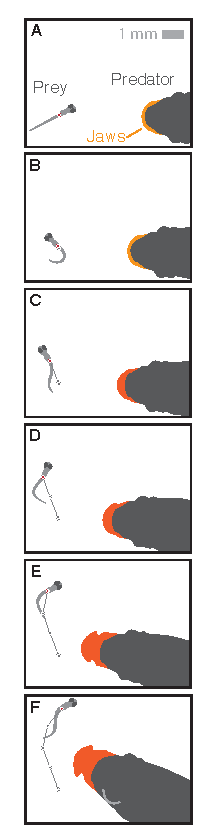
\includegraphics[width=.35\textwidth]{Fig_01.pdf}
\centering	
\caption{\textbf{A predator-prey interaction in zebrafish.} \textbf{(A)}  }
\label{pred_prey}
\end{SCfigure}


% FIG 2
\pagebreak
\begin{figure}[t]
\begin{centering}
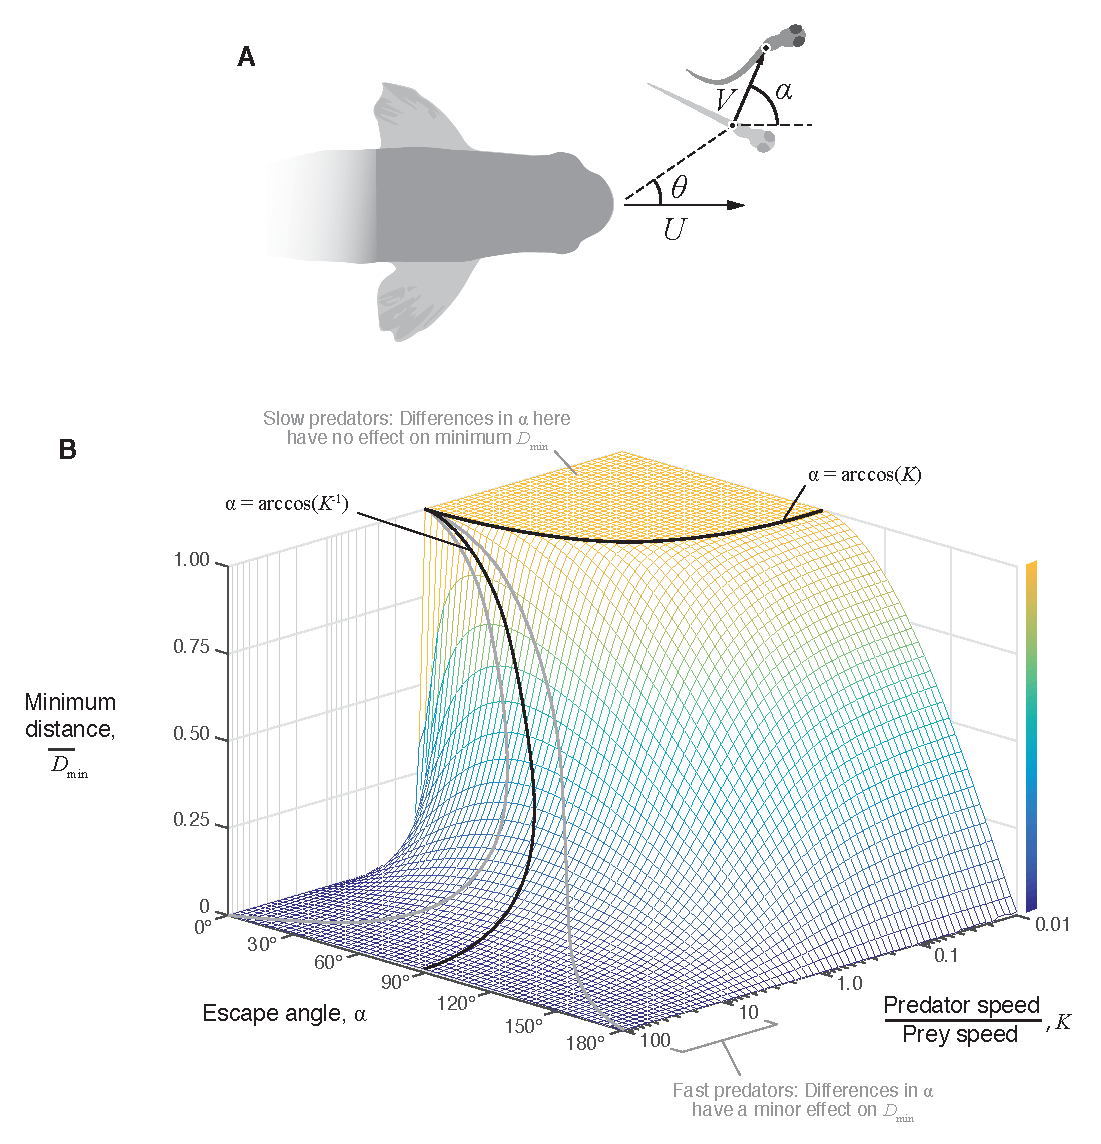
\includegraphics[width=1\textwidth]{Fig_02.pdf}
\centering	
\caption{\textbf{The Homicidal Chauffeur model, applied to prey strategy.} \textbf{(A)} Simulations predict the direction of a prey's fast start relative to initial position and velocity of a predator. \textbf{(B)} Numerical simulations were run at varying escape angle and predator approach speed to examine variation in the minimum distance. At $K>1$, the optimal angle. . .  }
\label{weihs_topo}
\end{centering}
\end{figure}



% FIG 3
\pagebreak
\begin{figure}[t]
\begin{centering}
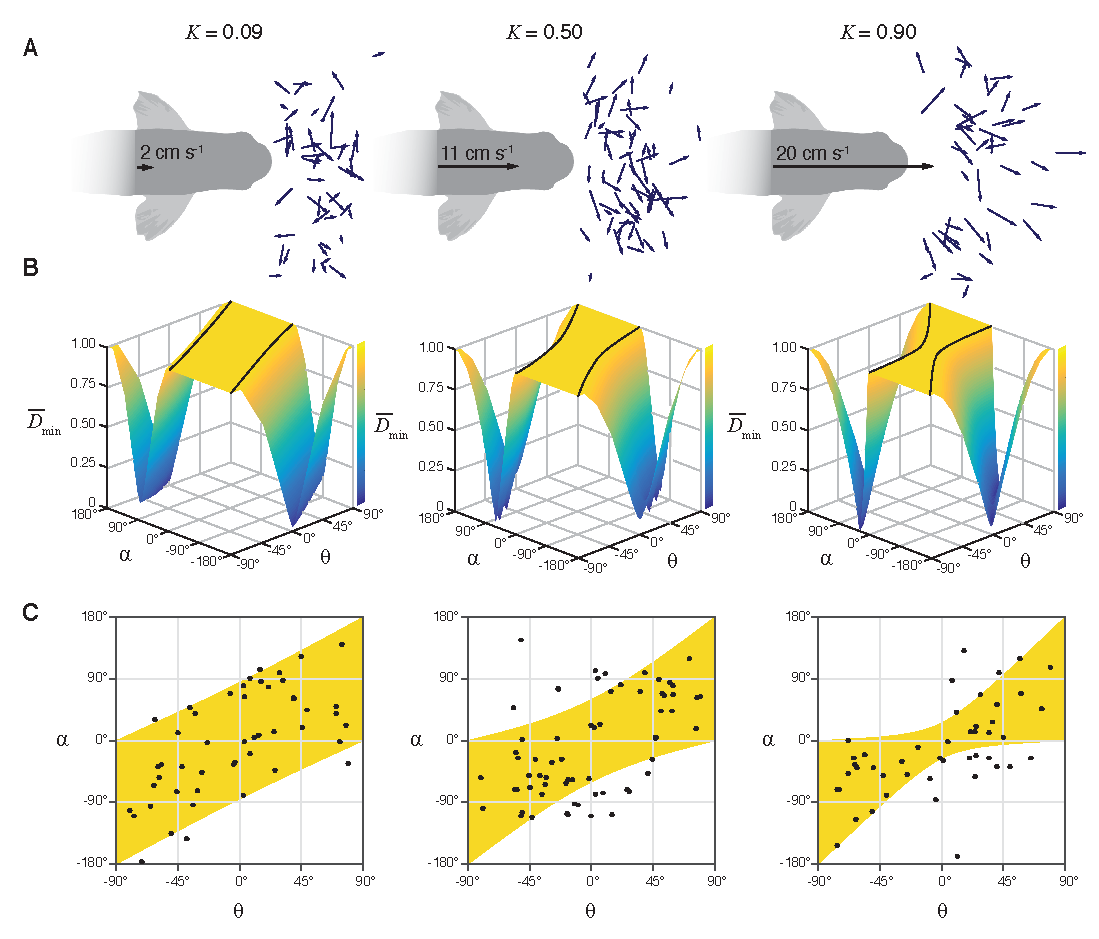
\includegraphics[width=1\textwidth]{Fig_03.pdf}
\centering	
\caption{\textbf{Model predictions and measurements of the fast start.} \textbf{(A)}  }
\label{our_topo}
\end{centering}
\end{figure}


% FIG 4
\pagebreak
\begin{figure}[t]
\begin{centering}
%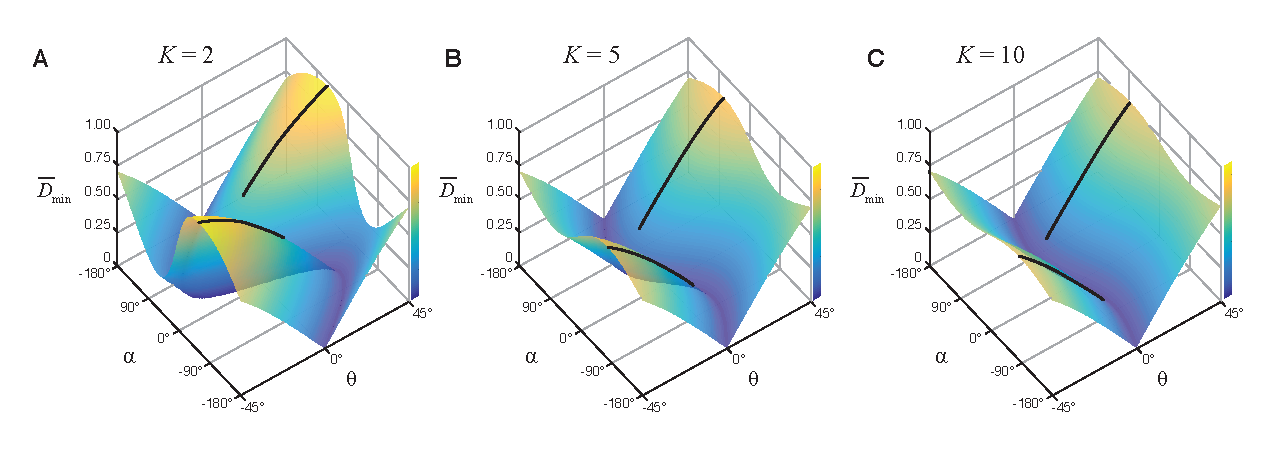
\includegraphics[width=1\textwidth]{Fig_04.pdf}
\centering	
\caption{\textbf{Model predictions and measurements of the fast start.} \textbf{(A)}  }
\label{k>1_topo}
\end{centering}
\end{figure}






% CLOSE DOCUMENT
\end{document}
